\documentclass[11pt]{article}
\usepackage[margin=1in]{geometry}
\usepackage{enumitem}
\usepackage{subcaption}
\usepackage{graphicx}

%opening
\title{CSCI 491/591, Project P5\\
		\small{Progress Report}}
\author{Group 8\\
		\small{Tao Huang and James Soddy}}
\twocolumn

\begin{document}

\maketitle

%Intro
For our project, our group has been investigating the shape of play by various
poker players. We started with the intention of exploring the space of poker
play, without any more specific aim than to find something interesting. As we
have worked on our project, our goal has solidified to attempt to find a 
relationship between the shape of a player's poker hands and their success
while playing those observed hands. We have had some degree of success in finding
shape in the data we have looked at, but the shapes are not as strong or as 
uniform as we would like. There are still some challenges ahead in finishing our
project, but we have a solid basis to present and write up if our remaining work
does not come up with stronger results.

\section*{Goals}
% Goals listed from P2
Our original goals, which we laid in our proposal, were to find a way to create
a shape which represented the play style of an individual player and to use those
shapes to find similarities and differences between players. In the proposal
we listed several objectives, which were:

\begin{itemize}[noitemsep]
	\item Define a topology which will give meaningful shape to the overall play
	for a given player.
	\item Create a method which will judge the difference between the shapes of
	each player's play
	\item Apply James' knowledge of poker to verify that the groupings our method
	defines seem reasonable.
	\item Be able to positively identify an individual player based on the
	'fingerprint' of the shape of their play
	\item Come up with some interesting and unexpected conclusions
\end{itemize}

We have made what we think is significant progress toward all of these
objectives, with the exception of positively identifying a single player. We have
set that goal aside, as our techniques have not come close to that level of
precision.

\section*{Initial Investigations}
Our initial work involved doing some research into poker, the types of different
play styles, and find some concrete metric we could compare our hands to.  We were
able to find some information about the primary differences in poker play styles,
as well as details about the value of different starting card combinations to the
player holding them. We thought we could use the play styles to help us interpret
any groupings among players that we might find in our analysis. We plotted the
starting hand values, in the hope that the resulting shape might be useful
as a comparison point for the shapes generated by actual players. (Shown in figure
1)

\begin{figure}[ht!]
		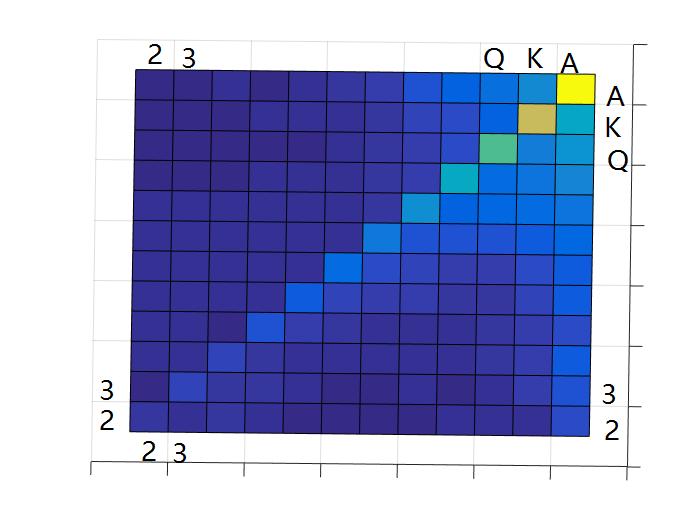
\includegraphics[width=.45\textwidth]{score}
  		\caption{\textbf{Heatmap of Poker Hand Values.} All possible differently 
  		valued starting Hold'Em hand combinations aligned in a grid, with 
  		their color indicating profitability (lighter is better)}
\end{figure}

We also
looked at academic literature to see if we could find work similar to ours which
we could apply. While we found academic papers on some aspects of poker, they
weren't topology related or particularly useful to our goals. We also found a
number of papers related to topology of games. Most of the topology papers dealt
with properties of special topological games, and of the remaining papers, there
were none which dealt with the topology of a player space or games with incomplete
information. So we needed to find our own techniques.

\section*{Hand Histories}
Another part of our work was dealing with the large number of hand history files
that we needed to extract data from. Our first step was to write a small perl
script which could parse the raw text files (example in figure 2) and retrieve
all of the information that we needed. The script created a file for each player
the first time they were encountered, and appended a new line for each hand the
player played in. On this line was each decision they made in the hand, as well
as what cards they had if that information was available. Once in this format,
the data would be easy to manipulate in any way we needed.

\begin{figure}[ht!]
		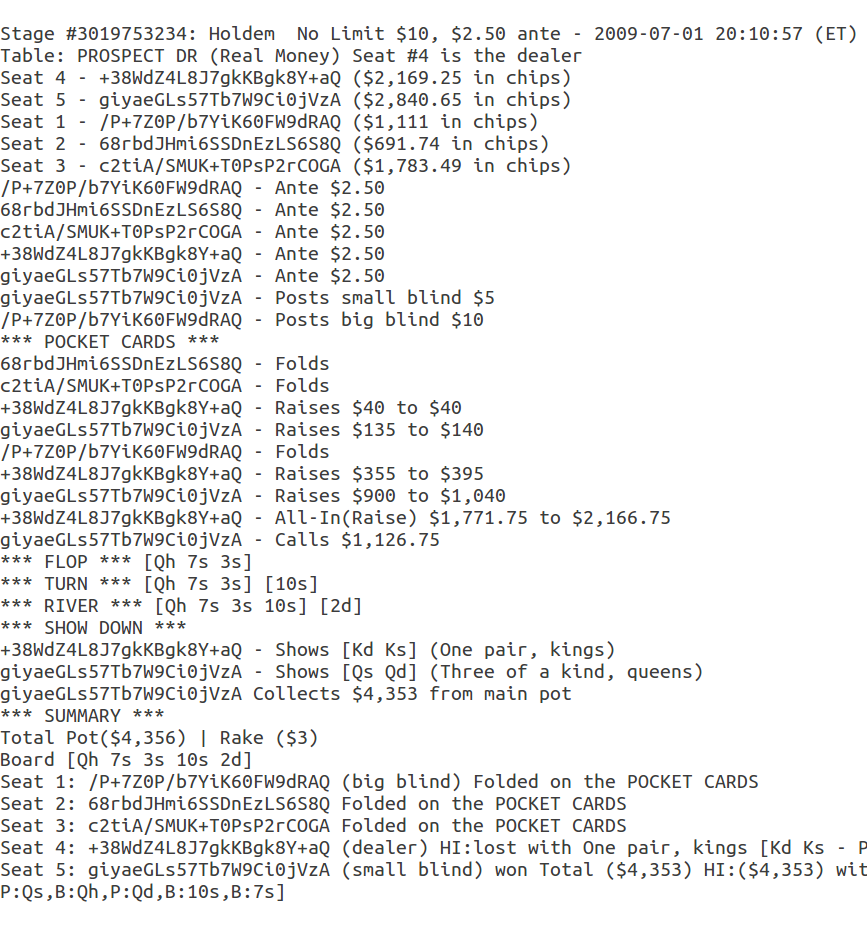
\includegraphics[width=.45\textwidth]{hand}
  		\caption{\textbf{Example hand.} One hand taken from the hand history files
  		we used in our project}
\end{figure}

\section*{Player Shapes}
Once we had our data in a manageable form, we needed to visualize it. We created
a second perl script which read the player files created by the first script and 
calculated the average amount of money they were willing to invest during the
first betting round with each possible starting hand. We then used MATLAB to
visualize these data in 2-dimensional and 3-dimensional pictures, similar to the
one we created for the starting hand values.

Looking at these charts, we were able to see clear patterns, and make some
conclusions about the players the charts had come from. Some of the charts which
were visually fairly similar to the starting hand value graphic belonged, as
expected, to the players who were winning at the highest rates. Also,
some of the shapes which bore little or no resemblance to the hand value shape
belonged to players with the heaviest losses. However, there was a great deal
of noise in the shapes, which we attributed mostly to the number of hands for each
player with hole card data available being very limited.

\section*{Distance}
Our next step was to attempt to find a useful way to measure the distance
between the shapes generated by different players. We partitioned our data into
two sets of hands for each player, so that we would have a way to compare check
that the shapes and distances actually said something about the players. Our
first attempt was to use a Hausdorff distance calculation package for R on our 
data. Unfortunately, we found that the distances calculated were not any closer
for our partitioned data than for shapes generated by completely different players.
This contradicted our principle that the techniques we use should return consistent
results.

We attempted several other metrics, and found our best results using a type of
$L^1$ norm on the data. Unfortunately, the average distance between the shape of
two partitioned sets from one player was still only about 25\% closer than the
distance between shapes from two unrelated players. The fact that we can see a
definite difference leads us to believe that our metric can be useful, but the
small magnitude of the difference makes it unhelpful for performing calculations
or coming to a better understanding of the data. We believe that if we had a larger
set of data with hole cards then we would be able to clean up some of the noise
and achieve more meaningful results.

%MDS

\section*{Future Work}
Currently, we are working to create a space of hands played based only on the
decisions made during the hand, and without any player card information
included. This is helpful because without the need to have players' hidden card
information, the number of hands we can use increases significantly. However,
the reason we have avoided this path is because it is much less clear how the
space should be defined. We hope to have this work done by the end of the week,
leaving us enough time to consider our results and include them in our final
report.

Some other work we still need to complete:

\begin{itemize}[noitemsep]
	\item Attempt a few more variations on our hidden-card shapes, such as
	removing zero points from the calculations, converting to a logarithmic
	scale, and working from a point cloud of all hands observed, rather than
	averaging them before doing calculations. This should be fairly straightforward
	and we should be complete on Saturday.
	\item We need to interpret our results, whether or not we are able to find
	any improved metrics before doing so. By Monday, April 25th we should have
	our analysis completed and know what we will be including in our reports.
	\item We will need to complete our presentation and final paper, detailing
	our experience and any results. This portion should be completed by Wednesday,
	April 27th at the latest.
\end{itemize}

\section*{Conclusion}
We have tried several different techniques to analyse our poker hand history data,
but have been somewhat disappointed with the results. We have been able to see
some interesting patterns and draw some conclusions, but we are still holding out
hope that we will have something stronger and more computable by the time we are 
done. While the tasks we still have to complete are significant, they are also
manageable and we feel good about our prospects for turning in an interesting
presentation and a quality paper.



\end{document}
